%\documentclass{sig-alt-release2}
%\documentclass{sig-alternate-2013}
\documentclass[12pt]{article}
\usepackage{graphicx}
\usepackage[T1]{fontenc}
\usepackage[nodayofweek]{datetime}
\usepackage{url}
\usepackage{color}
\usepackage{balance}

\usepackage{graphicx}
\usepackage{epstopdf}
\usepackage{subcaption}
\usepackage{url}

%from learning at scale:
\usepackage{graphicx}
\usepackage{epstopdf}
\usepackage{subcaption}
\usepackage{listings}
\usepackage[T1]{fontenc}
\usepackage[scaled=0.80]{beramono}
\usepackage{color}
\definecolor{bluekeywords}{rgb}{0.13,0.13,1}
\definecolor{greencomments}{rgb}{0,0.5,0}
\definecolor{redstrings}{rgb}{0.9,0,0}
\lstset{
showspaces=false,
showtabs=false,
breaklines=true,
showstringspaces=false,
breakatwhitespace=true,
escapeinside={(*@}{@*)},
commentstyle=\color{greencomments},
morekeywords = {MultiType},
keywordstyle=\color{bluekeywords}\bfseries,
stringstyle=\color{redstrings},
basicstyle=\ttfamily,
numbers=none, xleftmargin=.1in, numbersep=3pt
}

\usepackage{comment}

% create a shortcut to typeset table headings
\newcommand\tabhead[1]{\small\textbf{#1}}
% macro for code variables
\newcommand\codevar[1]{\texttt{#1}}


%\pdfpagewidth=8.5in
%\pdfpageheight=11in
%
%\begin{document}
%\conferenceinfo{ICER'13,} {August 12--14, 2013, San Diego, California, USA.}
%\CopyrightYear{2013}
%\crdata{978-X-XXXX-XXXX-X/XX/XX}
%
%
%\clubpenalty=10000
%\widowpenalty = 10000

\newfont{\mycrnotice}{ptmr8t at 7pt}
\newfont{\myconfname}{ptmri8t at 7pt}
\let\crnotice\mycrnotice%
\let\confname\myconfname%

%\permission{Permission to make digital or hard copies of part or all of this work for personal or classroom use is granted without fee provided that copies are not made or distributed for profit or commercial advantage, and that copies bear this notice and the full citation on the first page. Copyrights for third-party components of this work must be honored. For all other uses, contact the owner/author(s). Copyright is held by the author/owner(s).}
%\conferenceinfo{ICER'13,}{August 12--14, 2013, San Diego, California, USA.} \\
%\copyrightetc{ACM \the\acmcopyr\ ...\$15.00 \\ http://dx.doi.org/10.1145/2493394.2493421}
%\crdata{978-1-4503-2243-0/13/08}


%
%\clubpenalty=10000 
%\widowpenalty = 10000

\begin{document}

%\pagestyle{empty}
\title{Dealing with Multiple solutions of Design Problems: \\Mining Student-Generated Alternatives}

%\numberofauthors{1}
\author{Elena Glassman \\ MIT CSAIL \\ \textit{elg@mit.edu}
}

\maketitle

\begin{abstract}
This is an HCI approach to dealing with multiple solutions generated by students. Many coding problems have a specification that the student's solution must meet, but give the student a broad range of freedom for the internal design of that solution. There may be several distinct, correct solutions, some of which may be unknown to the teaching staff or intelligent tutor designer, making it potentially difficult for staff to help that student reach their own correct solution. My approach will be to visualize hundreds or thousands of student solutions to discover alternatives, and then classify the solutions, and the paths that students take to each solution, either by machine learning or human staff. The visualization and classifications will inform assistance given to students, in the form of staff-student discussions, peer-pairing, and/or automated help.

%Many coding problems, in the context of a course or online game, have a specification that the student's solution must meet, but give the student a broad range of freedom for the internal design of that solution. There may be several distinct, correct solutions, some of which may be unknown to the teaching staff or intelligent tutor designer, making it potentially difficult for staff to help that student reach their own correct solution. Visualization and classification of the multiple solutions that students generate in response to assigned engineering design problems will improve hints and answers to students' questions, whether they are provided by peers, staff, or automation. My approach will be to visualize hundreds or thousands of student solutions to discover alternatives, and then classify the solutions, and the paths that students take to each solution, either by machine learning or human staff. The classifications will inform assistance given to students, in the form of staff-student discussions, peer-pairing, and/or automated help.% I log incremental snapshots of students' solutions as they progress toward correct and incorrect solutions. Initial investigations demonstrate that the choice of features to represent solutions is critical, and may be domain- or problem-dependent. \textit{Rewrite to emphasize HCI approach.}
\end{abstract}

%\category{K.3.2}{Computers and Education} {Computers and Information Science
%  Education} [Computer Science Education]. See \cite{acm_classification:2013} for help using the ACM classification system.
%\terms {Measurement, Experimentation}
%
%\keywords{Choose your own specific keywords.}

%\category{K.3.2}{Computers and Education}{Computer and Information Science Education}[computer science education]
%
%\keywords{Problem Solving Process, Pattern Recognition}

%add categories about design-trade-offs, online learning, digital design
%\terms{Measurement, Performance, Human Factors} %Theory}
%\keywords{Pattern Recognition} %Problem Solving Process, Classification, Clustering, Intelligent Tutor, Student Progress Model, Similarity Metrics, Visual Data Mining, Programmer Event Data} %ACM proceedings, \LaTeX, text tagging}


\section{INTRODUCTION}

%I am a doctoral candidate in MIT's Electrical Engineering and Computer Science (EECS) Department. I have completed all of my qualifying exams, and am now in my fourth year. I discuss my initial thesis research investigations with several professors, including my advisor, Rob Miller. Together, they cover the fields of machine learning, human computer interfaces, and instructional design. I intend to formalize the relationship by the end of this summer, with the submission of my thesis proposal. I plan to analyze and present the data I collect from students over the next two years, in order to graduate in May 2015.

Many coding problems, in the context of a course or online game, have a specification that the student's solution must meet, but give the student a broad range of freedom for the internal design of that solution. There may be several distinct, correct solutions, some of which may be unknown to the teaching staff or intelligent tutor designer. This raises problems for helping students and giving feedback. In face-to-face situations, if a teaching assistant doesn't recognize the student's solution path, then they may redirect the student completely, costing them work and possibly derailing a novel, valid solution. In an intelligent tutor or massively open online course (MOOC), the automated hint generators may not recognize the unexpected solution paths, and will generate unhelpful hints.

This research aims to first develop tools and principles that support teachers' knowledge of the design space their students inhabit. This knowledge can enhance teachers' in-person interactions students, by inspiring conversations about alternative design possibilities. This knowledge can also inform teacher-trained classification algorithms that automatically identify and send feedback and guidance to particular students. The feedback and guidance would be written by the teachers in response to particular types of solutions, but once classifiers can reliably identify those types of solutions, the same feedback and guidance can be applied to other current students, and to future students. These solution-classifiers could also inform peer-pairing, when students must help one another.

I first will discuss related work from the fields of active (machine) learning, computer science education, and the learning sciences. I will then explain the chosen thesis problem, and describe the research methods selected for creating a solution to this problem. Interspersed with these research methods will be the descriptions of preliminary experiments which influenced the research method selections. Finally, I will conclude by laying out my expected contributions and a timeline for completion.

%In order to reduce confusion, I lay out a few definitions. In this proposal, I define an solution to be piece of code that a particular person wrote. I define a solution to be more abstract than an solution: while there may be an solution submitted by each student in the class, there may be only two distinct solutions, representing two different approaches or strategies to achieving the same input-output behavior. I define an solution path to be a series of code snapshots generated by a person working toward meeting a particular input-output behavior specification. Likewise, I define a solution path to be more abstract, referring to a general path that one or several solution paths may trace out on the way to a working solution. The ``space of student solutions'' refers to the aggregation of student-generated solutions and the variety of solutions they represent.
%
%There is a growing set of recent papers documenting methods for discovering the space of student-generated solutions. A common goal of this existing research is to help teachers monitor the state of their class, or enable them to give solution-specific feedback to more students. The proposed work will contribute to that literature, as well as explore how it can be integrated with other systems, such as peer-assistance platforms and automated help.


 %In the Matlab challenge, visualizing code parse tree size provides insight into common strategies as well as successful and unsuccessful outliers. 
%

%In CompArch, this led to better education of the teaching staff. As a result, I now ask a simple question to identify the student's approach before trying to help them.

%\section{MOTIVATING EXAMPLE}
%I am currently an instructor for an undergraduate introductory course on computer architecture (CompArch). Enrollment has swung between roughly two hundred and over three hundred students per semester. One mid-semester lab assignment in this course requires that students create state-transition rules for a Turing machine. %Each line in the behavioral specification boils down to the following: if you're in state \textbf{X} and you read symbol \textbf{Y} on the tape, overwrite symbol \textbf{Y} with symbol \textbf{Z}, move the tape-reader in direction \textbf{W}, and transition to state \textbf{Q}.
%Many distinct sets of state-transition rules behave identically, given the same input tape. %Even after looking at hundreds of Turing machines, which all give the same correct final answers, there is very little a human can discern simply by looking at the students' code. The same is true even after translating these textual statements into a diagram of state transitions.
%
%The dynamic behavior of students' Turing machines has recurring patterns. I visualized this dynamic behavior for 148 students' two-state Turing machines, and by visual inspection of the Turing machine's movement across a common input tape, identified strategies \cite{ICERGlassman}. The majority (88\%) of the solutions employed one of two mutually exclusive strategies: (1) matching the innermost open parenthesis with the innermost closed parenthesis and (2) matching the $n^{th}$ open parenthesis with the $n^{th}$ closed parenthesis.
%
%The fact that there were {\em two} correct solutions to the Turing machine assignment came as a surprise. I now ask struggling students a question first, to determine the solution they are aiming for. I can then suggest edits that preserve the chosen solution, if I recognize it as correct. Common solution identification also allows me to recognize novel alternative solutions.
%
%%Each staff member for this course is encouraged to complete the lab on their own before counseling students. Staff members were aware of the solution they each found, and yet were not aware that there were two mutually exclusive common solutions. 
%
%This is one example of an engineering design problem where a small number of common, distinct, correct solutions are distinguishable once an appropriate representation of the data is found. My thesis research explores the generality of this phenomenon, with a focus on scaling up to environments with hundreds or thousands of students.


\section{BACKGROUND \& RELATED WORK}

%I partitioned the related work based on method of discovering the space of solutions and existing structures within learning environments that this knowledge could enhance. The specific domain to which these methods and interventions are applied is noted as each reference is discussed. 

%The work highlighted in the first section below addresses the feasibility and current state-of-the-art in classifying student solutions and solution paths, using machine learning algorithms and visualization methods. The second section highlights work from the Computer Science Education community on the relevance of solution space knowledge to various methods used within learning environments. %The final subsection surveys the existing domains in which these methods have been applied, specifically concerning the type and scale of programming challenges.

Since terminology across research domains can vary, I will define the terms in which I will describe previous research and my own: 
\begin{itemize}
\item A solution is code that a particular person wrote in response to a prompt or problem description.
\item Solution clusters represent different patterns of implementation. For example, there may be two distinct solution clusters, both achieving the same input-output behavior but by different means. 
\item An solution path is a series of code snapshots generated while a person is working toward meeting a particular input-output behavior specification. 
\item The ``space of student solutions'' refers to the aggregation of student-generated solutions and the solution clusters they form.
\end{itemize}

\subsection{Comparing and Contrasting Examples}


Marton et al.'s variation theory \cite{Marton13} holds that in order to learn something, one must see examples that vary along particular dimensions: ``contrast,'' as in pairing it with something it is not; ``generalization,'' as in presenting multiple instances of the object or concept to be learned, varying only that which is irrelevant; ``separation,'' as in presenting multiple instances of the object or concept, varying only that which can vary internally without changing the object or concept into something else; and ``fusion,'' as in seeing multiple examples in which previously analytically separated aspects must be processed together to recognize the object or concept. The aspects which are related to these dimensions of variation and therefore define the object or concept are called ``critical features.''

Peer reviews and assessments, surveyed in \cite{peerReview98}, are one of the existing pedagogies in which teachers ask students to compare and constrast examples. The pedagogical method of comparing and contrasting ways of approaching a solution has now been validated in the literature of mathematics education research \cite{Star07}, cognitive science \cite{loewenstein2003analogical,kurtz01learning,telling}, and computing education research \cite{Suhonen08, PatitsasICER13}.

Given Marton et al.'s rubric for effective patterns of variation, and the identification of ``critical features,'' one can discern between more or less theoretically effective examples of the object or concept given to a student to learn. On this basis, Luxton-Reilly et al. \cite{Luxton13} suggest that identifying distinct clusters of solutions can help instructors select appropriate examples of code for teaching purposes. 

While this research has focused on the effects of multiple, varying examples on student learning, it is also, as suggested by Luxton-Reilly et al. \cite{Luxton13}, helpful for teachers' own understanding and quality of feedback and guidance. Facilitating the discovery or identification of critical features, which are possibly both teacher-specific and task-specific, is a major challenge I will address in this thesis.

\subsection{Thematic Analysis/Grounded Theory}

\textcolor{red}{Explain what it is}

Luxton-Reilly et al. \cite{Luxton13} takes this approach to discovering the kinds and degree of variation between student generated solutions that fulfilled the specifications of short introductory programming exercises in Java. By thematic analysis \cite{thematic06} of student submissions, the authors generated a taxonomy that captures the variation between correct solutions in their dataset. They created an Eclipse plug-in for classifying new code examples based on their taxonomy. \textbf{Make plugin description concrete and accurate}

\subsection{Mathematical Modeling Applied to Solutions}

\subsubsection{Supervised ML}

Taherkhani et al. \cite{taherkhani12} demonstrated the practicality of identifying which sorting algorithm a student implemented, using supervised machine learning methods. \textbf{Details! Features? Methods?}

\subsubsection{Unsupervised ML}

The most recent relevant work on finding clusters in solutions comes from Stanford. Huang et al. \cite{MOOCshop} consider tens of thousands of solutions submitted to Stanford's Fall 2011 Machine Learning MOOC, and identify clusters of solutions based on measures of syntactic and functional similarity. They make a case for mapping out the solution space using analysis beyond just input-output behavior. They claim that output-based feedback alone is insufficient, since the relationship between input-output pairs and bugs, both mental and programmatic, is not a one-to-one mapping. For students' approaches to implementing regularized logistic regression, similarly behaving programs were implemented in significantly different ways. 

\subsubsection{Active Learning/Interactive ML}

\textcolor{red}{EXPLAIN WHAT IML IS, BASED ON IML COURSE INTRO LECTURE.}

An active/interactive machine learning technique, which take advantage of human experts in the loop to resolve uncertainties, have been deployed for de-duplication in Stonebraker et al.'s Data Tamer \cite{DataTamer} and in a cardiac EGG-based alarm system\cite{JWiens}. \textcolor{red}{DETAILS.}

\subsubsection{Probabalistic Approaches}

Using automated classification methods, Piech et al. \cite{Piech} found distinct development paths students take to achieve working solutions that fulfilled the specifications of short introductory programming exercises in Java. Students' incremental paths were classified by pipeline that included milestone discovery, Hidden Markov Modeling of the students' process, and clustering of solution paths. These identified paths are visualized as finite state machine transition diagrams. The evaluation focused on predicting midterm exam grades and detecting milestone difficulty. \textbf{What did it contribute?}

Sudol et al.'s new metric, Probabilistic Distance to Solution, and its successful application to introductory programming exercises, is a second example of the feasibility of classifying and mapping out distinct paths to solutions \cite{sudol12}. \textbf{What exactly did she do, and what did it contribute?}

\subsubsection{Learning Students' Process and Behavior}

The following examples highlight research that is further from relevance to this thesis because the paths to a working solution are classified by behavior rather than the type of final solution found. Kiesmueller et al. \cite{Kiesmueller} attempted to recognize strategies at a very high level, which are not specific to the challenge at hand. Example high-level problem-independent strategies were a top-down or bottom-up programming style. Helminen et al. \cite{ICERHelminen} introduced novel interactive graphs for examining the problem solving process of students working on small programming-like problems. However, problems with multiple solutions were outside the scope of their investigation.



%
%\subsubsection{Active Learning of Solution Clusters}
%
%CITE DATA TAMER APPLICABILITY FOR ITS HUMAN ACTIVE LEARNING COMPONENT to partial solutions
%Community source the distance metrics/cluster boundaries: Ask Student: "Is this what you did?" Ask teacher: "Are these the same?"

%\subsection{Relevant Learning Environment Methods}




%More concretely, comparing and contrasting solution approaches Patitsas et al. \cite{PatitsasICER13} has 
%
% These methods have their theoretical basis in variation theory \cite{} and social cognitive theory \cite{}. 
%
%Comparing and contrasting dierent solution approaches is
%known in math education and cognitive science to increase
%student learning { what about CS? In this experiment, we
%replicated work from Rittle-Johnson and Star, using a pretest{
%intervention{posttest{follow-up design (n=241). Our intervention was an in-class workbook in CS2. A randomized half
%of students received questions in a compare-and-contrast
%style, seeing dierent code for dierent algorithms in parallel. The other half saw the same code questions sequentially,
%and evaluated them one at a time. Students in the former
%group performed better with regard to procedural knowledge (code reading & writing), and 
%exibility (generating,
%recognizing & evaluating multiple ways to solve a problem).
%The two groups performed equally on conceptual knowledge.
%Our results agree with those of Rittle-Johnson and Star, indicating that the existing work in this area generalizes to CS
%education.
%
%In light of these pedagogical frameworks, Luxton-Reilly et al. \cite{Luxton13} suggest that identifying distinct clusters of solutions can help instructors select appropriate examples of code for teaching purposes.


%\textbf{insert transition to next section}
\subsection{Feedback to Students}

Peer-pairing can stand in place of staff assistance, to both reduce the load on teaching staff and give students a chance to gain ownership of material through teaching it to someone else. Weld et al. speculate about peer-pairing in MOOCs based on student competency measures \cite{WeldHcomp12}, and Klemmer et al. demonstrates peer assessments' scalability to large online design-oriented classes \cite{Klemmer}.

Generating tailored feedback to students in large classes tackling problems even as short as introductory programming assignments requires many man-hours of repetitive work. Singh et al. \cite{rishabh} are pushing the state of the art of automated feedback for short introductory programming assignments. However, their software is currently only differentiating between solutions based on their input-output characteristics. For example, this system cannot currently differentiate between two different sorting algorithms. If there are common dead-ends that have been identified by looking at incorrect student solutions to a particular problem, by hand, this system can identify that a student is very close to a known dead-end approach, but it cannot identify {\em which} functionally equivalent variant of a correct solution a student is approaching. 

Singh et al.'s automated feedback represents the one end of the spectrum for providing tailored feedback to students because hints are algorithmically generated; Huang et al. \cite{MOOCshop} represents the other end, by ``force multiplying'' human-generated feedback. By clustering syntactically similar solutions which fail on the same input-output tests, Huang et al. aim to enable the sending of appropriate teacher-written feedback to entire clusters of solutions.

%\subsection{Domain of Application}
%
%LOOK AT COMPARCH COMMUNITY, describe scale of Singh solution, MOOCshop solution, types of programming (languages)

\section{STATEMENT OF THESIS/PROBLEM}

Visualization and classification of the multiple solutions that students generate will improve hints and answers to students' questions, whether they are provided by peers, staff, or automation. 

I plan to explore the following aspects of this claim:
\begin{itemize}

\item What features are useful for visualizing or automatically classifying alternative solutions?

\item How do we facilitate teachers' understanding of the design space generated by students?

\item How do we get students to think about alternatives not taken?

\item How can peers help each other when there are multiple good solutions?

\item How can we provide automated help based on archived solutions?

%\item What features are useful for visualizing or automatically clustering engineering design solution paths? For programming domains, for example, features could include measures of program complexity, stack depth, and runtime characteristics. For digital logic and analog circuit domains, features could include graph metrics and voltage traces on intermediate nodes.
%\item How can teaching staff be trained to quickly recognize the solution path of a given student, in order to give tailored feedback?
%\item If teaching staff are in short supply (as in a MOOC), how can peers help each other in a space where there are multiple good solution paths?
%\item If peer help is not feasible, then how can we provide automated help based on solution path recognition in a design space where multiple correct paths are possible?
\end{itemize}


\section{RESEARCH GOALS \& METHODS}

The approach will be to visualize hundreds or thousands of student solutions to discover alternatives, and then classify the solutions, and the paths that students take to each solution, either by machine learning or human staff. The classifications will inform assistance given to students, in the form of staff-student discussions, peer-pairing, and/or automated help.

%\subsection{Enabling Exploratory Data Analysis and Clustering}

\subsection{Exploratory Data Analysis}

As a researcher, my first step toward discovering the space of correct solutions for a given assignment will be to look at the raw data. I have access to anonymized code submissions from the Spring 2013 semester of both a virtual hardware (6.004) and software (6.005) design class. I also have access to submissions to an online Matlab programming game, python submissions to Introduction to Computer Science and Programming (6.00x), and also potentially the python submissions of Introduction to Electrical Engineering and Computer Science I (6.01). 

By poring over many examples of students' code, I can get a sense for what design decisions partition the space of implemented solutions into useful clusters. Useful, in this case, refers to clusters which help me conceptualize the space of solutions and identify where new students fall into that space. 

I have also given randomly chosen subsets of solutions to teaching staff or knowledgeable experts, for clustering by hand. By studying the ways in which humans, given the same set of solutions, come up with different partitions of the solution space, I can assess which features I need in order to support any or all those distinctions. 

I have already taken this approach to an assignment in 6.004, an undergraduate computer architecture course in which virtual hardware is designed at the MOSFET and CMOS gate level and coded in a variant of SPICE called JSIM. Note that, when looking at raw JSIM code submissions to 6.004, human-made clusterings had little relationship to basic measurements, like the number of MOSFETs instantiated. This is unsurprising, since solution size is not readily apparent when looking at the raw code submitted. When I clustered solutions while knowing their relative size, size was a very helpful variable for clustering, and contributed heavily to my mental model of the design space. The relationship between the representation of solutions, in the form of measurements or features, and the human's mental model built while examining solutions, is the first of several reasons why HCI is the approach being taken for this problem.

Regardless of the clustering(s) found, the intuition gained through this first exploratory step, akin to thematic analysis \cite{thematic06}, guide the steps that follow.

\subsection{Feature Engineering}

Feature engineering is a critical challenge; the ``critical features'' discussed in the learning sciences literature are not yet known, and may be domain, task, and teacher dependent. This is another reason for the HCI approach of this thesis: there will need to be a tight loop between the human, presumabely a member of the teaching staff, and the representation of the solutions, in order to extract meaning.

\subsubsection{Fingerprinting}

One strategy which has worked well for discovering similar code segments in larger pieces of source code is document fingerprinting \cite{MossFolks}, where functions of small sections of code are considered ``fingerprints.'' A fingerprint is constructed by computing hashes for all $n$-grams in a document (for some chosen $n$). Similar code will contain similar fingerprint components. In their algorithm for the MOSS plagiarism-detection system, AUTHORS \cite{MossFolks} introduce \emph{winnowing}, an efficient technique for generating fingerprints with a guarantee that identical code sections above a user-selected minimum size will always yield identical components in the fingerprint.

Unfortunately, fingerprinting is not well-suited to our goal of clustering similar solutions. Using the existence or absence of particular fingerprints in a solution as features for clustering has not provided good initial results on Java or JSIM code examples, as experienced by Max Goldman or myself. In Goldman's investigations with Java source code, even after removing irrelevant features such as variable names and considering token-level $n$-grams, the number of different $n$-grams was too large for unsupervised clustering to be effective. He hypothesizes that, while more similar documents are likely to have more similar fingerprints, the additional noise makes fingerprint similarity an unreliable distance metric for a clustering algorithm.


%We might instead put aside not only the idea of winnowing, but of selecting a compact fingerprint at all: while a fingerprint might normally be constructed by computing hashes for all $n$-grams in a document (for some chosen $n$) and selecting a subset of them, we can retain all the hashes. If we believe that dissimilar code will contain different $n$-grams in different amounts, we can use vectors in the space of $n$-grams to identify submissions. In our investigations with Java source code, however, even after removing irrelevant features such as variable names and considering token-level $n$-grams, the number of different $n$-grams was too large for unsupervised clustering to be effective.

\subsubsection{Function Calls, AST size, and Control Flow}

Working in collaboration with Singh, we now generate feature vectors for python programs that include the size of different sub-trees of the abstract syntax tree (AST), the control flow of the program, and the usage of python libraries and constructs. In total, we computed around $60$ features for the python programs, the details of which are listed in the Appendix. Some of these features include: number of program variables, number of conditional and loop statements, type of comparisons, number of AST nodes, the control structure of if-loop statements, number and type of library functions used etc.

Figure~\ref{comp-deriv-diff-attempts} shows a small sample of student attempts for the \codevar{comp-deriv} problem. The problem asks students to write a python function that returns the derivative of a polynomial whose coefficients are represented as a python list. The two student submissions in Figure~\ref{comp-deriv-diff-attempts}(a) immediately return [0.0] if the length of input polynomial is 1 (base case) , otherwise they return the computed derivative list after removing its first element. The two submissions use similar control flow structure, same number of \codevar{return} statements and the library function \codevar{append}, but use list splicing and \codevar{pop} library functions respectively for removing the first element from the derivative list. The two student submissions in Figure~\ref{comp-deriv-diff-attempts}(b) perform len(poly)-1 number of iterations first to compute the derivative list and then add [0.0] to the empty result for the base case. They again have similar control flow structure, same number of \codevar{return} statements, and similar \codevar{range} function usage. The student submission in Figure \ref{comp-deriv-diff-attempts}(c) shows a solution that computes the derivative list by popping elements out of the input list and returns when the length of input list becomes 1, whereas Figure~\ref{comp-deriv-diff-attempts}(d) shows a submission that uses list comprehension.



\begin{figure*}[!htpb]
\begin{tabular}{c|c|c}
\begin{minipage}{.32\linewidth}
\begin{lstlisting}[language=python]
def computeDeriv(poly):
    powers = len(poly)
    if powers == 1: 
        return [0.0]
    deriv = []
    for i in range(powers):
        deriv.append(poly[i]*i)
    return deriv[1:]
\end{lstlisting}
\end{minipage}
&
\begin{minipage}{.32\linewidth}
\begin{lstlisting}[language=python]
def computeDeriv(poly):
    ans = []
    for i in range(1,len(poly)):
        ans.append(i*poly[i])
    if ans == []:
        ans = [0.0]
    return ans
\end{lstlisting}
\end{minipage}

&
\begin{minipage}{.32\linewidth}
\begin{lstlisting}[language=python]
def computeDeriv(poly):
    idx = 1
    res = list([])
    if len(poly) == 1:
        return [0.0]
    while idx <= len(poly):
        coeff = poly.pop(1)
        res.append(coeff*idx)
        idx = idx + 1
        if len(poly) < 2:
            return res
\end{lstlisting}
\hspace*{30mm} (c)
\end{minipage}

\\

\begin{minipage}{.32\linewidth}
\begin{lstlisting}[language=python]
def computeDeriv(poly):
    if len(poly) > 1:
        res = []
    else: return [0.0]
    for i in range(len(poly)):
        res.append(poly[i]*i)
    res.pop(0)
    return res
\end{lstlisting}
\end{minipage}
&
\begin{minipage}{.32\linewidth}
\begin{lstlisting}[language=python]
def computeDeriv(poly):
    result = []
    for i in range(1,len(poly)):
        result.append(i*poly[i])
    if len(result) == 0:
        result.append(0.0)
    return result
\end{lstlisting}
\end{minipage}

&
\begin{minipage}{.32\linewidth}
\begin{lstlisting}[language=python]
def computeDeriv(poly):
      if len(poly) == 1:
        return [0.0]
    newList = [ poly[i] * i for i in range(1, len(poly))]
    return newList
\end{lstlisting}
\end{minipage}
\\
(a) & (b) & (d)
\end{tabular}
\caption{A sample of student submissions for the \codevar{comp-deriv} problem showing both similar and different implementations. (a) Two student submissions that immediately return [0.0] if the length of input polynomial is 1 (base case) and return the computed derivative list after removing the first element. (b) Two student submissions that perform len(poly)-1 number of iterations first to compute the desired derivative and adds [0.0] to the empty result in the end. (c) A student solution iterating by popping elements out of the input list and returning when the length of list becomes 1. (d) A student solution using list comprehension.}
\label{comp-deriv-diff-attempts}
\end{figure*}


\subsection{Visualization}

A next step toward discovering the space of correct solutions is visualizing many student solutions together. If the appropriate feature(s) are chosen, simultaneously viewing representations of hundreds or thousands of solutions to the same problem helps humans and machines extract of patterns. The choice of features and graphical representation is initialized by exploratory data analysis but highly influenceable by later results of machine learning algorithms and other mathematical modeling techniques. 

I have already taken this approach to multiple labs in 6.004. I have also observed this approach in a collaborator's work on an online Matlab programming challenge called Cody. Plotting dynamic behavior or static features such as parse tree size is enough, in these initial and relatively simple examples, to separate students' solutions into clear clusters representing different solutions. %Figure \ref{nedfigsAll} has been reproduced from our joint submission \cite{ICERGlassman} to a computing education research conference.

\subsubsection{Cody Solution Maps}
Solutions submitted to Cody are immediately evaluated and scored. Once the code is validated with a suite of input-output constraints, it can be displayed on a solution map. Two examples of solution maps are shown in Figures \ref{nedfig1} and \ref{nedfig2}. 
 
The solution map plots solutions as points against two axes: order of arrival (on the horizontal axis) and code size (on the vertical axis). Correct answers are green circles. Incorrect answers are red x's. We define \textit{code size} as the number of nodes in the parse tree of the solution. Despite the simplicity of this metric, code size can provide quick and valuable insight when assessing large numbers of solutions. An instructor is likely to be interested in common responses, both correct and incorrect, as well as extreme outliers, and the solution map reveals these and other interesting patterns.
 
For example, Figure \ref{nedfig1} shows a solution map for a problem which has a single obvious solution. Almost all the solutions are correct and exactly the same size. This presents as a great many correct solutions in a single line, packed so close together that they blur into a single rail of green circles.

When a problem has two common solutions, we might see two rails. Figure \ref{nedfig2} shows the solution map for the Triangular Number problem. The computationally efficient solution for the nth triangular number is $n(n+1)/2$. A less efficient but simple MATLAB solution is to create and then sum the series from 1 to n. These solutions are the two rails evident in this solution map for the Triangular Number problem.

\begin{figure*}[p]
\centering
\begin{subfigure}[b]{1.0\textwidth}
	\centering
%\includegraphics{fig1}
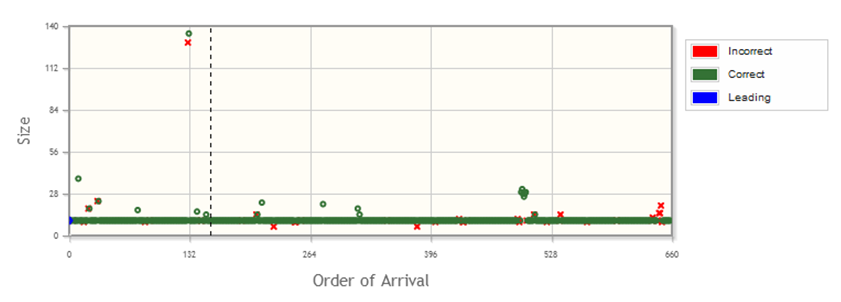
\includegraphics[scale=0.65]{nedfig1.png}
\caption{The solution map for a problem which has a single obvious solution.}
\label{nedfig1}
\end{subfigure}
\begin{subfigure}[b]{1.0\textwidth}
	\centering
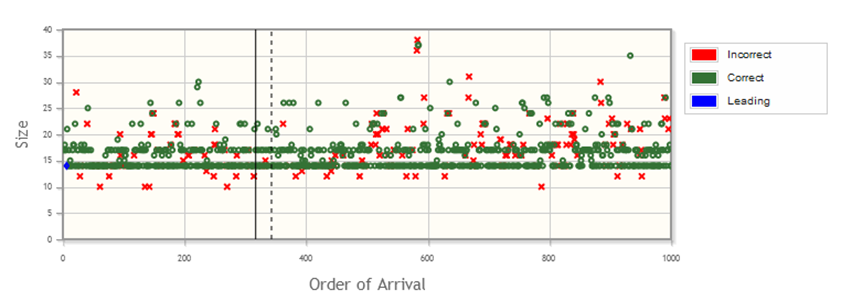
\includegraphics[scale=0.65]{nedfig2.png}
\caption{The solution map for a problem which has two common solutions.}
\label{nedfig2}
\end{subfigure}
\label{nedfigsAll}
\caption{Solution map examples. The \textit{leading} solution is the earliest, smallest correct solution.}
\end{figure*}

\subsubsection{Turing Machine Analysis}

The second example comes from 6.004, but is not coded in JSIM. Rather, it is coded in a custom language for describing the behavior of Turing Machines. The assignment requires that students write the state-transition rules for a Turing machine that halts on the symbol `1' if the input is a string of matched parentheses and halts on a `0' otherwise. Each student designs their own symbol library and state names for the finite state machine portion of their Turing machine, and lists behavior specifications. Each line in the behavioral specification boils down to the following: if you're in state X and you read symbol Y on the tape, overwrite symbol Y with symbol Z, move the tape-reader in direction W, and transition to state Q.

It is difficult to help students with the Turing machine assignment because many sets of state-transition rules behave identically, given the same input tape of parentheses. Even after looking at hundreds of Turing machines, which all give the same correct final answers, there is very little a human can discern simply by looking at the students' code. The same is true even after translating these textual statements into a diagram of state transitions.

Each staff member is encouraged to complete the lab on their own before counseling students. Staff members were aware of the solution they each found, and yet were not aware that there were two mutually exclusive common solutions. At least one staff member admitted steering students away from solutions they did not recognize, but in retrospect may have indeed been valid solutions.

In order to visualize this dynamic behavior, I ran all the two-state machines on the same test tape containing a string of open and closed parentheses. The movement of the tape-reading head across this input was logged in coordinates relative to the common starting point, at the left end of the test tape, and displayed along the vertical axis. The horizontal axis represents the number of steps taken by the Turing machine on its way to completing the task. These discrete steps are analogous to time. 

The majority (88\%) of the solutions employed one of two mutually exclusive strategies. These strategies were identified by visual inspection of the movement of many Turing machines across a common input tape. Figure \ref{turingFig} shows their locations on the common input tape over time, segregated by strategy into Figures \ref{tapeMoveA} and \ref{tapeMoveB}. These two strategies for determining whether or not the tape's string of parentheses is balanced are (1) matching the innermost open parenthesis with the innermost closed parenthesis and (2) matching the $n^{th}$ open parenthesis with the $n^{th}$ closed parenthesis, as is the case in standard mathematical notation. The remaining 12\% of solutions included less common strategies. At least two strategies in this group are known to pass the provided, fixed test suite but are wrong, because they cannot handle an arbitrary depth of nested parentheses. % are not general. %, shown in Fig. \ref{tapeMoveC}.

\begin{figure*}[p]
%\centering
%\includegraphics{fig1}
%\includegraphics[scale=0.85]{tmvisualization_InnerParensMatched_allkidsAnno}

\begin{subfigure}[b]{1.0\textwidth}
	\centering
%	
\includegraphics[width=0.65\textwidth]{ICERtapeLocations.png}
	
\includegraphics[width=140mm]{ICERtapeLocations.png}
	\caption{Tape on which all 148 two-state Turing machines were tested, and the numbering system by which locations along the test tape are identified.}
	\label{tapeLocations}
\end{subfigure}

\begin{subfigure}[b]{1.0\textwidth}
                \centering
                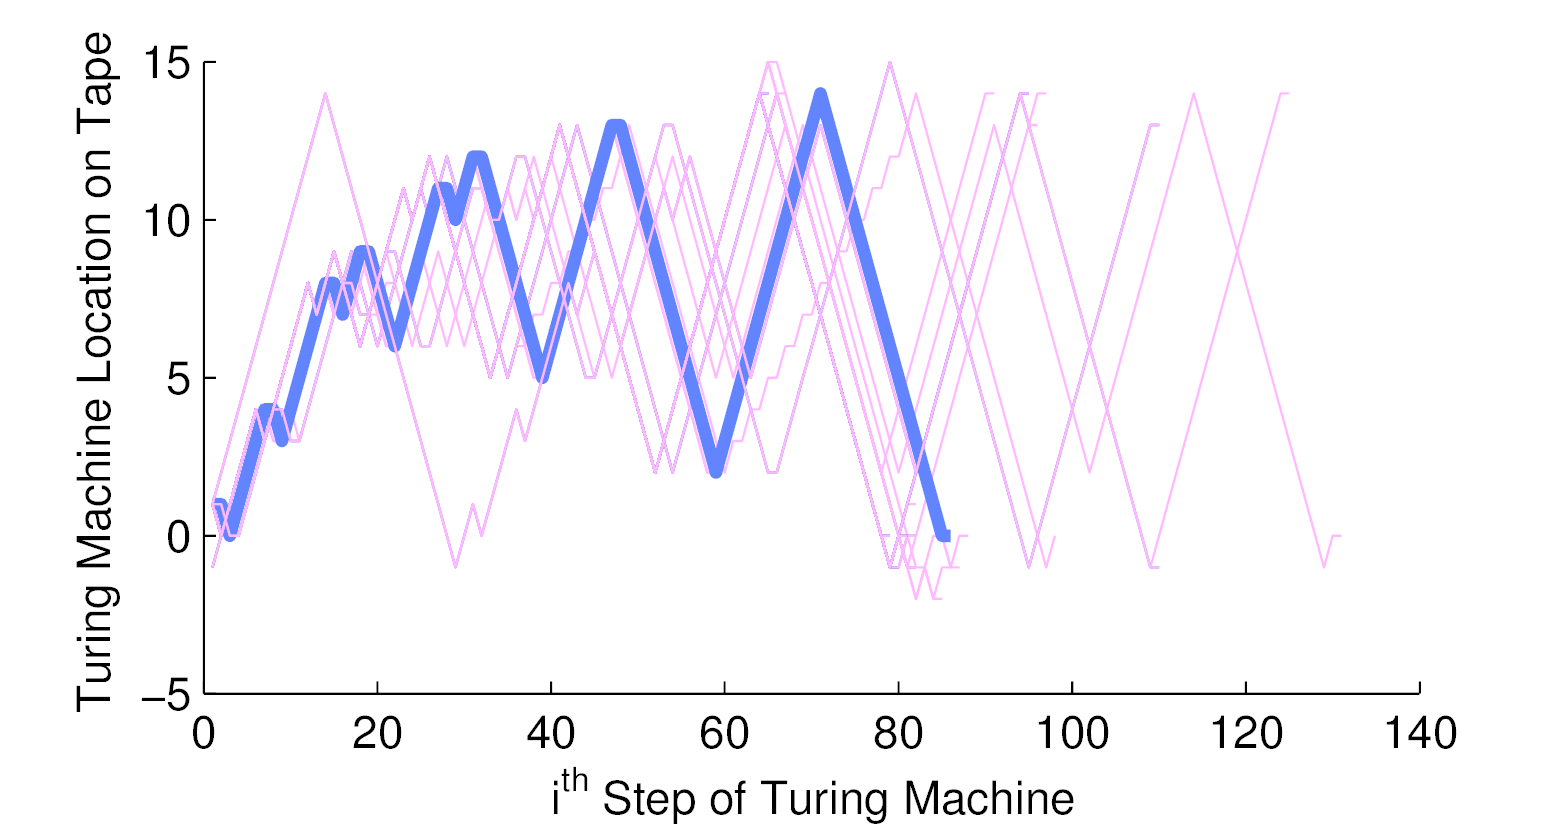
\includegraphics[width=0.85\textwidth]{tmvisualization_InnerParensMatched_allkidsAnno2}
%\caption{Cluster A: Of the 148 two-state Turing machines run on the common test tape \\ '( ) ( ( ) ( ( ( ) ) ( ) ) )', the trajectories of the tape reading heads of the 73 Turing machines which paired inner sets of open and closed parenthesis, as is standard in mathematical notation, are shown above as Cluster A. In this figure and those that follow in which trajectories are overlaid, the frequency of each variant is not visible. The bold trajectory represents a particularly clean example.}
\caption{Strategy A Turing machines: those which paired inner sets of open and closed parentheses, as is standard in mathematical notation. (73 out of 148 Turing machines)}
\label{tapeMoveA}
\end{subfigure}
%\includegraphics[scale=0.85]{tmvisualization_NtoNParensMatched_allkidsAnno}
\begin{subfigure}[b]{1.0\textwidth}
                \centering
                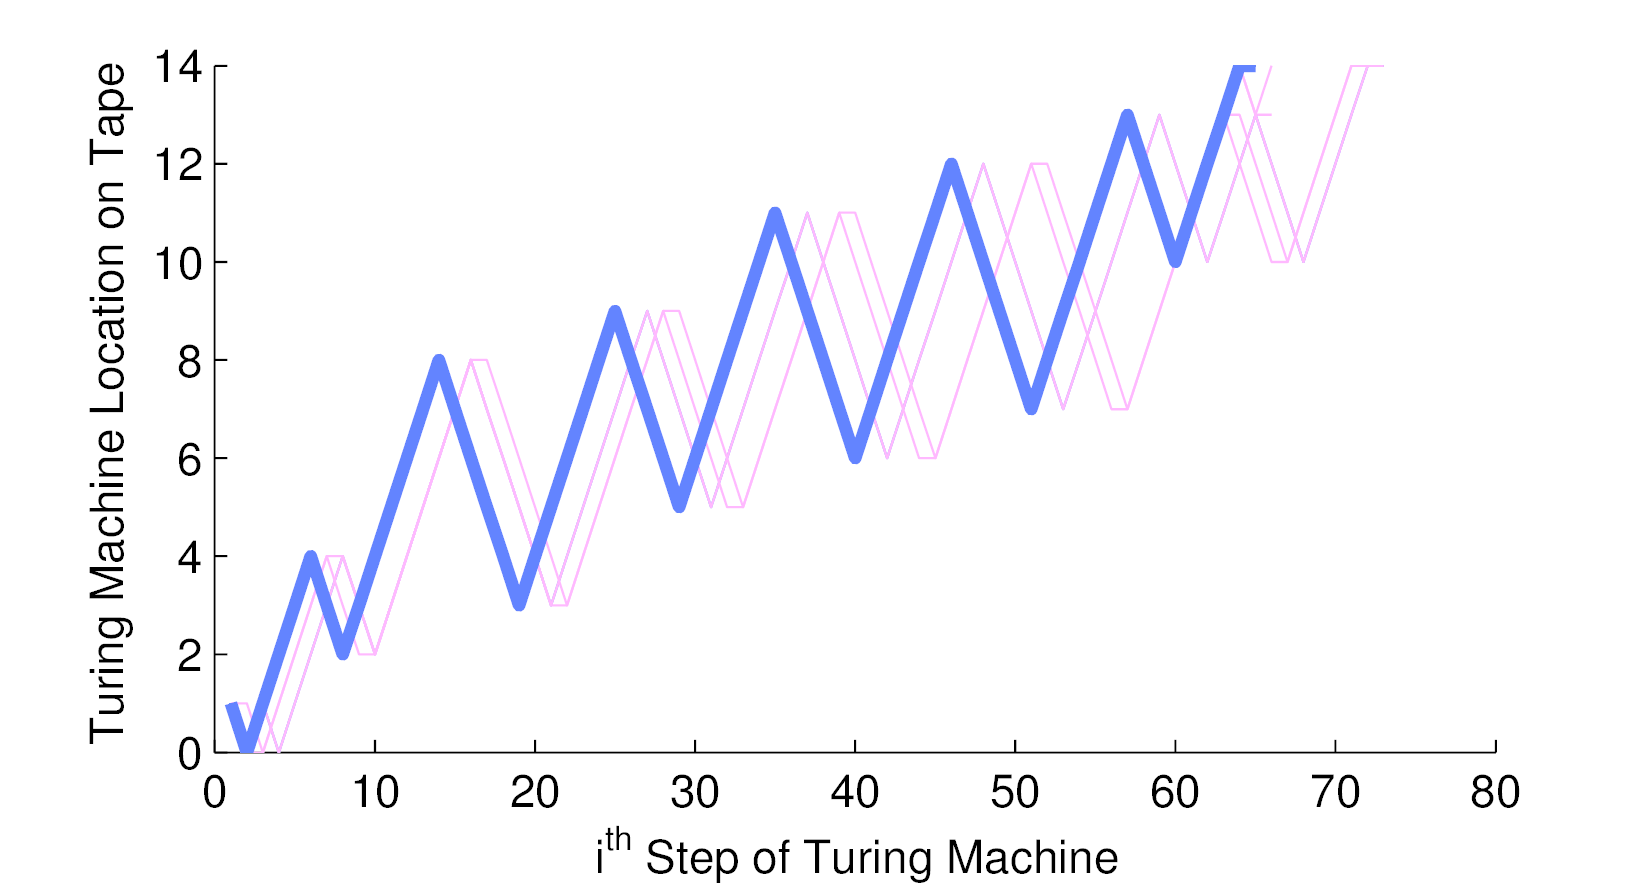
\includegraphics[width=0.85\textwidth]{tmvisualization_NtoNParensMatched_allkidsAnno2}
%\caption{Cluster B: Of the 148 two-state Turing machines run on the same common test tape \\ '( ) ( ( ) ( ( ( ) ) ( ) ) )' as above, the trajectories of the tape reading heads of the 58 Turing machines which paired the first open with the first closed parenthesis, and the second open with the second closed parenthesis, are shown above as Cluster B. The bold trajectory represents a particularly clean example.}
\caption{Strategy B Turing machines: those which paired the first open with the first closed parenthesis, the second open with the second closed parenthesis, etc. (58 out of 148 Turing machines)}
\label{tapeMoveB}
\end{subfigure}
%\includegraphics[scale=0.85]{tmvisualization_Other_allkidsAnno}
%\caption{The trajectories of the 17 remaining Turing machines, run on the same common test tape as above, which have yet to be categorized. Both bold trajectories correspond to solutions that do not work in general, but passed the provided, fixed test suite.}
%\label{tapeMoveC}
\caption{The two most common strategies for a two-state Turing machine to determine if a string of parentheses is balanced. Figures \ref{tapeMoveA} and \ref{tapeMoveB} show tape head position over time on the tape illustrated in Fig. \ref{tapeLocations}. The bold trajectories represent particularly clean examples.}
\label{turingFig}
\end{figure*}

\subsubsection{Analysis of a 4-Bit Adder Construction Lab}

My third example also comes from 6.004. From submission logs of the Spring 2013 semester, I studied students’ final correct solutions, which are implementations of a CMOS circuit that performs addition on two unsigned 4-bit numbers and produces a 5-bit result. This assignment is coded in JSIM, the hardware description language similar to SPICE. These circuits are created by students declaring internal nodes connected by P- and N-type MOSFETs in an appropriate topology. The students’ programming environment includes a simple editor for entering a circuit description and a waveform browser to view the results of a simulation. Nearly two hundred students submitted correct implementations of the 4-bit adder. 

It is suggested in the assignment’s lab handout that students first build a library of logic gates, such as NAND, NOR, XOR, and XNOR, out of N- and P-FETs. From that library of logic gates, the lab describes how to build the logic gates that compute the sum and carry bits of a 1-bit adder, also called a full adder. The lab pictorially represents how these full adders can be chained together to form one 4-bit ripple carry adder circuit, as shown in Figure. \ref{allFullAdders}.

One can see in the histogram of solutions by size, quantified by the number of MOSFETs instantiated in the simulated device, shown in Figure \ref{4bitAdders}, that there is a major cluster, several smaller clusters, and multiple solution size outliers, large and small. On closer examination of the solutions in each of these peaks, the tallest peak represents two similar but distinct solutions, one of which is a direct transcription of the assignment's description into JSIM code. The smallest solutions represent students who have identified intermediate nodes that can be shared by multiple subcircuits. By identifying and removing redundant nodes, students produced small, difficult-to-read circuits. Students who produced relatively large solutions instantiated unnecessary gates and/or used ``positive logic'' rather than inverting logic. Since CMOS gates can only implement inverting functions like NAND and NOR, additional inverters are necessary to make ANDs and ORs. To create solutions with positive logic, students composed AND and OR gates, and chained them together, rather than reasoning about how to chain NANDs and NORs together to implement the same function.

%\textbf{Describe visualizations of Lab2 solutions}

\begin{figure}
%\centering
\begin{subfigure}{1.0\columnwidth}
\centering
%\includegraphics{fig1}
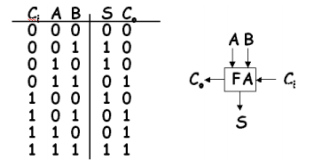
\includegraphics[scale=0.45]{fullAdderAndTruthTable.png}
\caption{The truth table for the sum and carry bits of a full adder component.}
\label{fullAdderAndTruthTable}
\end{subfigure}
\begin{subfigure}{1.0\columnwidth}
	\centering
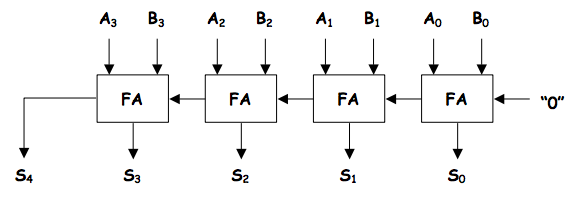
\includegraphics[scale=0.45]{chainedFullAdders.png}
\caption{The chain of full adders that forms the ripple-carry 4-bit adder.}
\label{chainedFullAdders}
\end{subfigure}
\caption{A ripple-carry 4-bit adder.}
\label{allFullAdders}
\end{figure}

\begin{figure}
%\centering
%\begin{subfigure}{1.0\columnwidth}
%\centering
%%\includegraphics{fig1}
%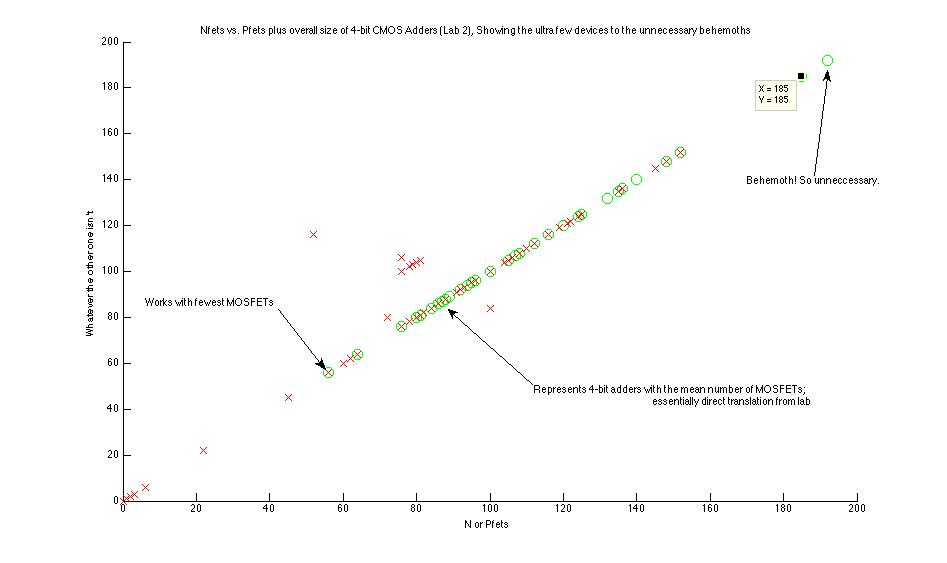
\includegraphics[scale=0.45]{nvspfets_lab2.png}
%\caption{\textcolor{red}{Fill in description}}
%\label{4bitadderslabeled}
%\end{subfigure}
%\begin{subfigure}{1.0\columnwidth}
%	%\centering
%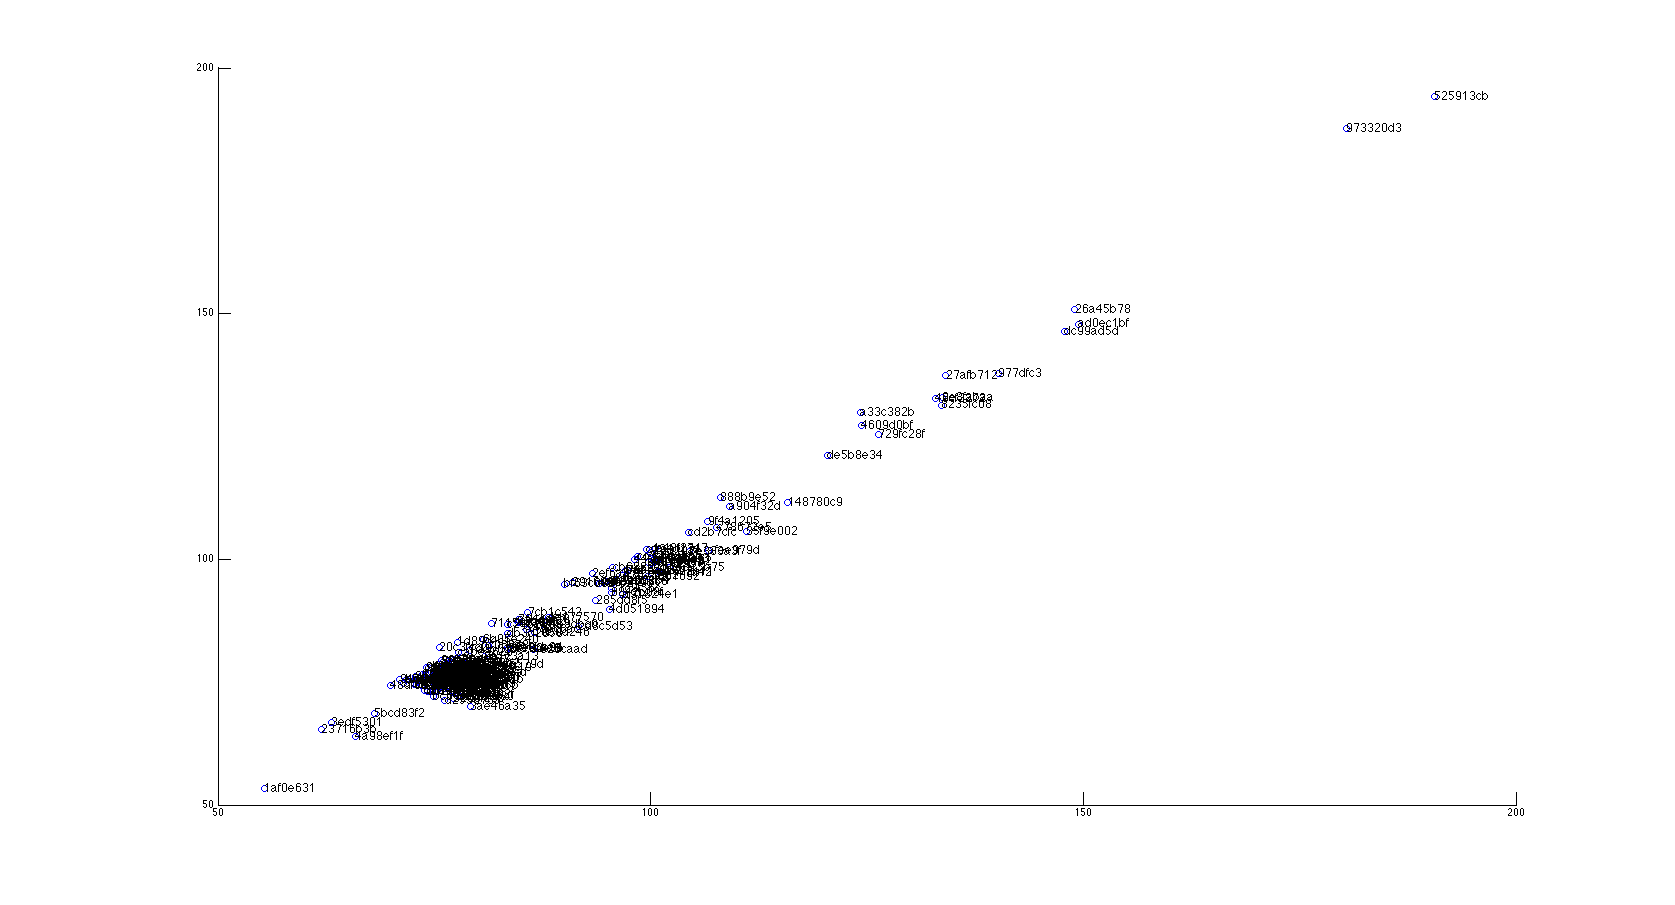
\includegraphics[scale=0.3]{matlabVizLab2.png}
%\caption{\textcolor{red}{Fill in description}}
%\label{4bitaddersjittered}
%\end{subfigure}
\centering
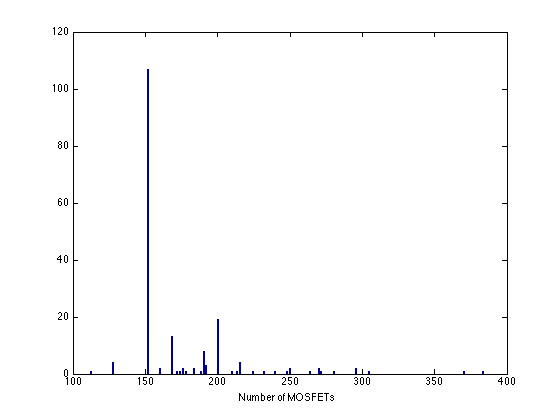
\includegraphics[scale=0.8]{histOfTotalCircuitSizeLab2.png}
\caption{Histogram of ripple-carry 4-bit adders.}
\label{4bitAdders}
\end{figure}


\subsection{Mathematical Modeling}

Once feature vectors are composed for each solution in a dataset, it is possible to apply machine learning and other mathematical modeling techniques to cluster the data or otherwise extract relationships between solutions and between features. As an initial exploration of feasibility, Rishabh Singh and I applied an unsupervised clustering method to 6.00x Python submissions. 6.00x is a Massively Open Online Course, or MOOC, that serves as an introduction to programming.

Singh obtained thousands of submissions to the course exercises during the Fall 2012 course offering. We filtered out all incorrect submissions, as indicated by input-output testing, so that we could focus on variations in correct solutions. The number of correct submissions analyzed for each problem is shown in Table. \ref{table-edx-probs}. The MOOC platform provided a web-interface for students to write and test their code in the browser itself, and students were provided 30 attempts to submit their solutions for each of the exercises.

\begin{table}
\begin{tabular} {|c|c|c|}
\hline
\tabhead{Problem Description} & \tabhead{Total Submissions} & \tabhead {Correct Submissions} \\ \hline
\codevar{comp-deriv} & 3013 & 1433 \\ \hline
\codevar{hangman-guess} & 1746 & 1118 \\ \hline
\codevar{iter-power} & 8940 & 3875 \\ \hline
\end{tabular}
\caption{Dataset of 6.00x problems from Fall 2012.}
\label{table-edx-probs}
\end{table}

The \codevar{comp-deriv} and \codevar{hangman-guess} problems were part of week 3 problem set exercises, whereas \codevar{iter-power} was an in-lecture exercise for the lecture on iteration. The \codevar{comp-deriv} problem requires students to write a python function to compute the derivative of a polynomial, where the coefficients of the polynomial are represented as a python list. The \codevar{hangman-guess} problem takes a string \codevar{secretWord} and a list of characters \codevar{lettersGuessed} as input, and asks students to write a function that returns a string where all letters in \codevar{secretWord} that are not present in the list \codevar{lettersGuessed} are replaced with an underscore. The \codevar{iter-power} problem asks students to write a function to compute the exponential $\codevar{base}^\codevar{exp}$ iteratively using successive multiplication.


\subsection{Human-Computer Interaction}

After repeating this process on several domains and tasks within those domains, including 6.004's design assignments written in a hardware description language and 6.00x's software designs written in Python, I propose to generalize the experience and build a tool for teachers which supports this kind of exploratory analysis of student solutions regardless of the teachers' specific domain and assignment. The eligible space of domains this could potentially generalize to are ones in which solutions are submitted as machine-readable code and where assignments have a specification that the student's solution must meet, but give the student a broad range of freedom for the internal design of that solution.

The exploratory data analysis and feature selection will power machine learning tools, such as clustering algorithms, potentially including active/interactive machine learning modules for teachers to correct the systems' classification of new solutions. 

\subsubsection{Evaluation}

In order to evaluate the contribution of this interactive data visualization environment for teaching staff, I will run a user study on staff members of courses, at MIT and possibly other institutions, in which the student submissions are in machine-readable code and there is non-trivial latitude given to students for the internal solution design. By interacting with representations of many students solutions' at once, users will attempt to identify clusters. If staff independently find similarly meaningful, persistent patterns in their students' solutions using the tool, I will consider it a success. I will also follow up with qualitative interviews with course staff who did and did not use the tool, about their understanding of the space of solutions to a particular assignment they are aware of, after the conclusion of that assignment.

\subsubsection{Adaptation for Students}

Inspired by both the literature on the educational value of comparing and constrasting alternative designs, as well as a personal desire to incorporate higher level discussions of design choices and trade-offs into CompArch, among other classes, I will adapt the teacher-targeted exploratory data analysis and visualization tool into a student-targeted explanatory data visualization tool. This tool will show students where their solution lies in the space of solutions. The role of this visualization will be to serve as a rich conversation piece over which students and staff, and also eventually student pairs and small groups, can discuss design decisions and solutions that are alternatives to their own. 

One measure of the success of this tool will be to quantify the accuracy and comprehensiveness of short written statements comparing and constrasting students' own solutions with other solutions. If the accuracy and comprehensiveness of self-reflective statements are higher when a student can interact with the visualization tool than when students are given a portfolio of printed out raw code examples to leaf through, then I can conclude that the visualization provides student-accessible information.

\subsection{Solution Path Recognition}

%In CompArch, we capture snapshots of students' intermediate code as they work. One semester's data has been collected already. 

As of the beginning of the Spring 2013 term, the CompArch course software now saves complete snapshots of student solutions-in-progress whenever a student saves or runs tests. Over the course of these snapshots, each solution-in-progress evolves into a complete solution employing one of possibly several distinct, correct strategies. Informative features of partial solutions would enable supervised machine learning algorithms to successfully predict which strategy a particular solution-in-progress will evolve toward. I hope to demonstrate generality on similar datasets from 6.005, a software engineering course which also has collected snapshot sequences of students' code.

%When it is not. However, if common strategies have already been identified from analysis of previous students' solutions, a teacher could hand-write a multiple choice question or two inquiring at a high level about the strategy of the student. This extends from the solution-space-informed question I now ask help-seeking students working on the CompArch Turning Machine Lab \cite{ICERGlassman}.

Solution path recognition can inform peer-pairing. There are a variety of possible solution path-dependent pairing strategies; however, the most straightforward strategy to employ first is to pair students whom the system predicts are on {\em similar} paths to a solution. By comparing metrics of students' progression toward a solution when paired based on solution paths, relative to random pairing and no pairing, I can measure the interventions' effect on the completion of the current lab and subsequent related labs.

Solution path recognition can inform automated forms of assistance as well. By incorporating all known solutions as reference solutions in Singh et al's AutoGrader \cite{rishabh}, the authors of that work believe it may be possible to overcome its current inability to consider which distinct solution an solution is closest to. Alternatively, code differences between a code snapshot in an unfinished solution path and the nearest code snapshot that belongs to a completed path may be a more simple form of automated help when a student has exhausted all other resources. % in addition to input-output behavior.

%My approach will be to visualize hundreds or thousands of student solutions to discover alternatives, and then classify the path that students take to each solution, either by machine learning or human staff. The classifications will inform assistance given to students, in the form of staff-student discussions, peer-pairing, and automated help. 

%There are three main variables within this thesis. The first is domain, as in whether the data is generated by a hardward or software course, and the scale of student implemementations. The second variable is the method of classification: are humans interpreting visualizations or are machine learning algorithms doing the bulk of the classification. Finally, there is the application of this generated knowledge. It can be used to facilitate design review discussions between staff and students, pair peers, or improve automated feedback.

%I will run a user study to access whether the interactive data visualization environment I design helps teaching staff find meaningful strategy distinctions. My subjects will be teaching staff of engineering courses. If subjects use the tool and find similar demarcations between strategies, and possibly similar sets of features to describe those demarcations, it may be possible to conclude the tool itself is enabling the staff to identify meaningful, persistent patterns in their students' solutions. %In a pre- and post-interview, we can analyze how the tool affects the staff's understanding of the ways in which a student can solve a particular assigned engineering problem.



% The learning, satisfaction, and perception of self-efficacy gains associated with these pairing strategies can be tested in a study deployed within a residential or online engineering class, after integrating the existing question-and-answer/discussion forum with the learning management system that keeps track of each student's solution paths.

%For example, one could pair two students whose solution paths are heading toward the same solution among the multiple possibilities for a particular engineering design problem, but one has a bug that the other has already fixed in their own code. Alternatively, one could pair two students, one who has already successfully employed a particular strategy with one who is struggling to implement it. The learning, satisfaction, and perception of self-efficacy gains associated with these pairing strategies can be tested in a study deployed within a residential or online engineering class, after integrating the existing question-and-answer/discussion forum with the learning management system that keeps track of each student's history of solutions. By incentivising students to assist other students, and then pairing them randomly or according to solution path-dependent strategies, I can approximately measure the educational value of the intervention.
%
%

\section{EXPECTED CONTRIBUTIONS}

\textcolor{red}{I hope to discover the qualities of critical features of coding assignments in the course of this research, and a process by which teachers can identify specific critical features in their own settings.}

%This research may be particularly helpful to staff who focus on helping each student reach their own envisioned solution. The algorithms, tools, visualizations, and resulting insights from this work are intended to support this constructivist approach to teaching, facilitate students helping each other, and inform automated feedback.

There are two end-users of the proposed software systems. I expect to create a software which helps teachers across multiple domains discover the full space of alternatives and recognize novel or better solutions in their students' solutions. I also expect to build software that help students understand alternative design choices and their tradeoffs, and reach their envisioned (valid) solutions.

While the tangible deliverables will be specific instances of software, I will report on the generalizability of visualization and classification of the multiple solutions as a tool for improving hints and answers to students' questions, whether they are provided by peers, staff, or automation. I will also report on the character of ``critical features'' found to be helpful for understanding the space of solutions, the methods by which students were brought to reason and comprehend design alternatives, and how peers can be effectively paired within a space where individual solutions can vary widely.

%I plan to explore the following aspects of this claim:
%\begin{itemize}
%
%\item What features are useful for visualizing or automatically classifying alternative solutions?
%
%\item How do we get students to think about alternatives not taken?
%
%\item How can peers help each other when there are multiple good solutions?
%
%\item How can we provide automated help based on archived solutions?

%Since my thesis research is relevant to engineering design tasks with multiple correct solutions, it may be of particular interest to teaching staff with a constructivist perspective. Such staff members may be attempting to elicit the student's envisioned solution strategy, and then help them toward a working solution that employs that strategy. The algorithms, tools, visualizations, and resulting insights from this and future work are intended to augment this constructivist approach to teaching, facilitate students helping each other, and inform automated feedback.

\section{TIMELINE}

\begin{itemize}
\item {\bf Fall '13} Deploy server-based D3 visualizations of working student submissions in the context of last years' working submissions during check-offs with me in 6.004. Log interactions with the visualization and record conversations with students while they compare their design to other options. Explore the generalization of the visualizations to representing Java exercises completed in 6.005 during past semesters. Explore use of Rishabh Singh's autograder for JSIM, and note what gaps in feedback arise from its current sole consideration on input-output behavior.
\item {\bf Spring '14} Use Bose Fellowship to improve and deploy visualization web applications for all interested LAs and TAs, interviewing them on their knowledge of the solution space pre- and post-interaction with the visualization. Add machine learning components as necessary, for helping humans identify patterns. Explore use for partial as well as completed labs. Iterate with 6.005 staff on visualizations of Java exercises that suit their course and classroom needs. Work with Singh to augment his autograder so that it gives feedback informed by which of several solutions a student is "closest" to.
\item {\bf Summer '14} Do an internship outside Boston, probably focusing on the visual presentation of information.
\item {\bf Fall '15} Use Bose Fellowship to improve and deploy visualization web applications for all interested LAs and TAs, and auto-suggest peer-pairings for students based on partial solutions. Compare solution paths for students experiencing auto-suggested peer assistance versus staff assistance. Continue iterating with 6.005 staff on visualizations of Java exercises that suit their course and classroom needs. Deploy Singh's modified autograder in 6.004.
\item {\bf Spring '15} Write thesis. Tie up loose ends. Defend thesis. Celebrate. Graduate!
\end{itemize}

\section{Acknowledgments}
This work is supported by the National Science Foundation Graduate Research Fellowship under Grant No. 1122374 and the MIT Amar Bose Teaching Fellowship. It has also been made possible by countless discussions and pair-research sessions with fellow members of CSAIL HCI, Prof. Leslie Kaelbling, Prof. Chris Terman, and Marty Glassman.

\bibliographystyle{abbrv}
\bibliography{icerbib}

%\bibliographystyle{abbrvurl}
%%\bibliography{biblio} Edit the name of your bib file here and delete the refs below.
%\begin{thebibliography}{1}
%\bibitem{acrobat_reader:2013}
%Adobe {A}crobat {R}eader 7.
%\newblock URL: \url{http://www.adobe.com/products/acrobat/}.
%\bibitem{acm_classification:2013}
%How to {C}lassify {W}orks {U}sing {ACM}'s {C}omputing {C}lassification
%{S}ystem.
%\newblock URL: \url{http://www.acm.org/class/how_to_use.html}.
%\bibitem{anderson:1992}
%R.~Anderson.
%\newblock Social impacts of computing: Codes of professional ethics.
%\newblock {\em Social Science Computing Review}, 10(2):453--469, 1992.
%\end{thebibliography}
\end{document}

